\section*{CHAPTER 4: SYSTEM IMPLEMENTATION AND RESULTS}
\addcontentsline{toc}{section}{\numberline{}CHAPTER 4: SYSTEM IMPLEMENTATION AND RESULTS}
\setcounter{section}{4}
\setcounter{subsection}{0}
\setcounter{figure}{0}
\setcounter{table}{0}

This chapter describes the practical implementation of the theoretical designs discussed in Chapter 3. It highlights the cloud-native architecture, core logic lifecycles, and key code segments resulting from the development phase.

\begin{figure}[htbp]
    \centering
    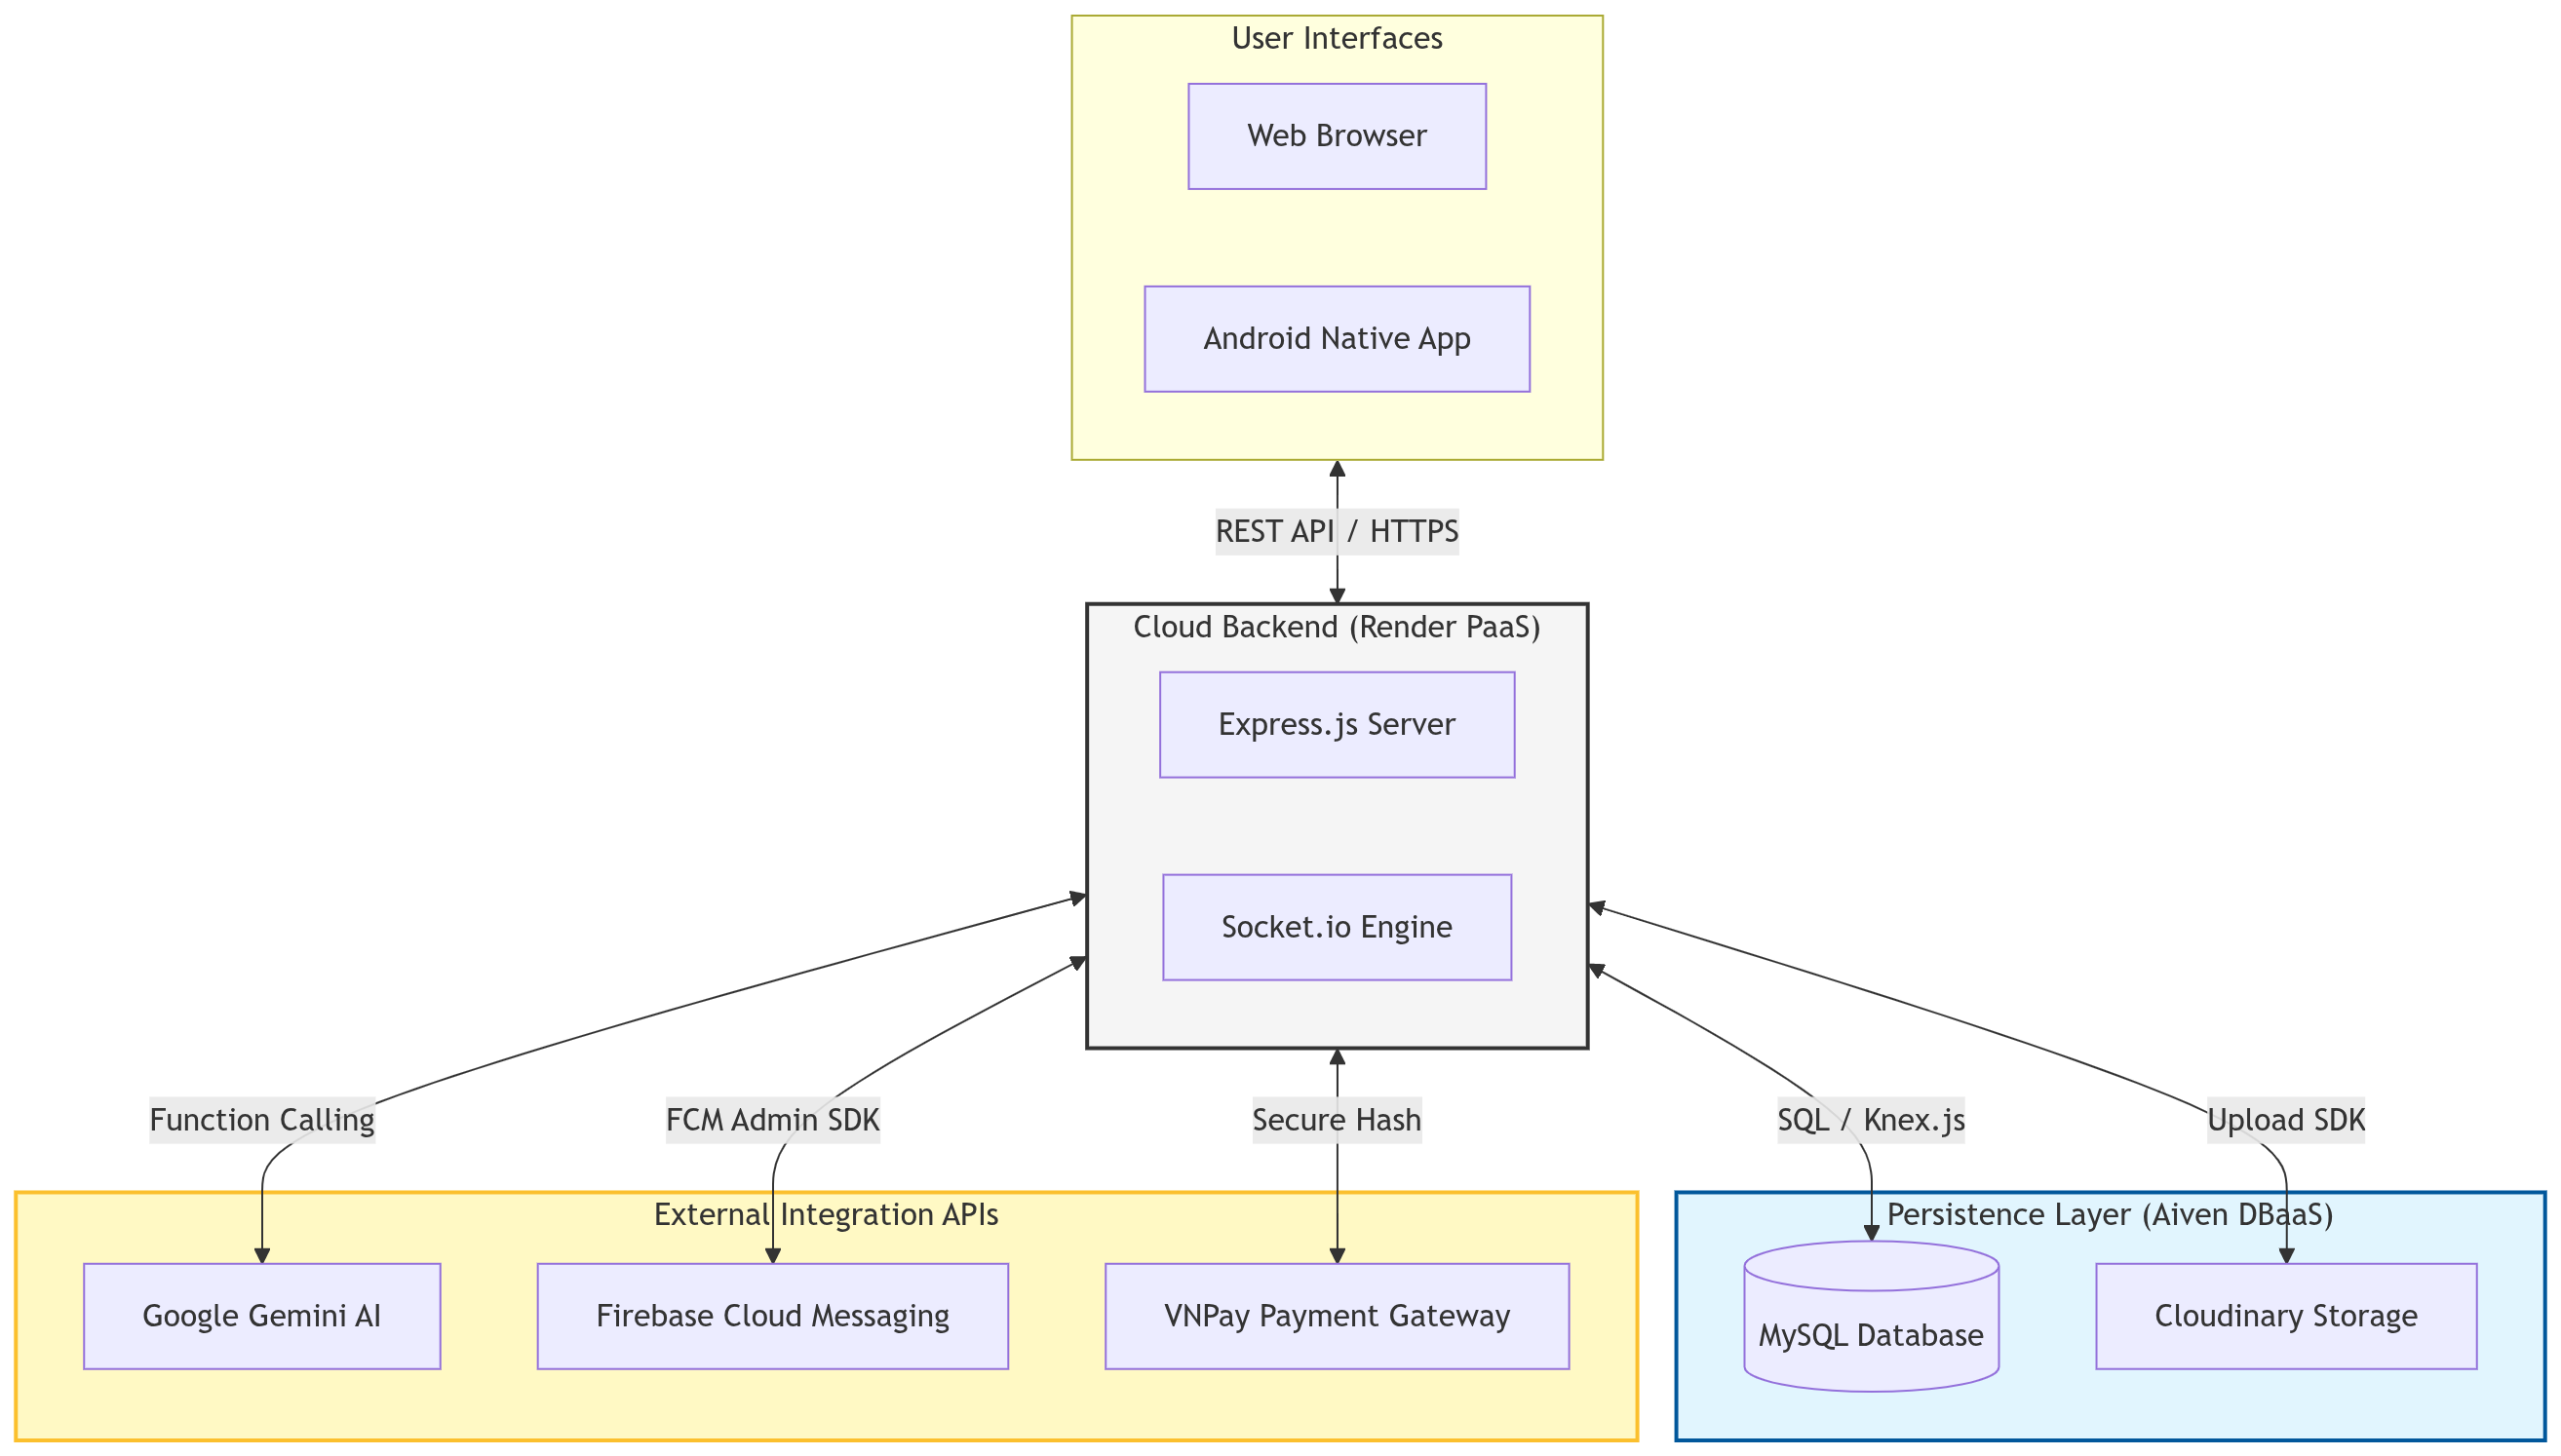
\includegraphics[width=1\textwidth]{Figures/system_architecture.png}
    \caption{Full-stack Multi-tenant SaaS Architecture with External Integrations}
    \label{fig:arch}
\end{figure}

\subsection{Backend Architecture Implementation}
The backend is structured using a Model-View-Controller (MVC) inspired pattern adapted for a RESTful API service. The \texttt{src} directory is logically divided into \texttt{routes}, \texttt{controllers}, \texttt{services}, and \texttt{models}.

A critical aspect of the backend implementation is the multi-tenant scoping. Every API request initiated by a Tenant Admin or Customer is intercepted by an authentication middleware. This middleware extracts the \texttt{tenant\_id} from the session or URL parameters and injects it into the request context. 

When querying the database using Knex.js, the models strictly enforce the tenant boundary. For instance, retrieving the list of fields for a tenant is implemented as:
\begin{verbatim}
// src/models/Field.js
class Field {
  static async findByTenant(tenantId) {
    return db('fields').where('tenant_id', tenantId);
  }
}
\end{verbatim}
This simple yet highly effective pattern guarantees that no tenant can access data belonging to another, forming the backbone of the SaaS security model.

\begin{table}[htbp]
\centering
\begin{tabularx}{\textwidth}{|l|l|X|l|}
\hline
\rowcolor{LightCyan}
\textbf{Endpoint Path} & \textbf{Method} & \textbf{Description} & \textbf{Access} \\ \hline
\texttt{/api/auth/login} & POST & Authenticates users and issues session tokens. & Public \\ \hline
\texttt{/api/chatbot/query} & POST & Processes natural language queries via Gemini AI. & Customer \\ \hline
\texttt{/api/fields} & GET & Retrieves field list filtered by \texttt{tenant\_id}. & Tenant/Cust \\ \hline
\texttt{/api/payment/vnpay} & POST & Generates secure VNPay payment URLs. & Customer \\ \hline
\texttt{/api/checkin} & POST & Validates QR codes and updates booking status. & Tenant Admin \\ \hline
\end{tabularx}
\caption{Core Backend API Endpoints and Access Control Policies}
\label{tab:api_endpoints}
\end{table}



\begin{figure}[htbp]
    \centering
    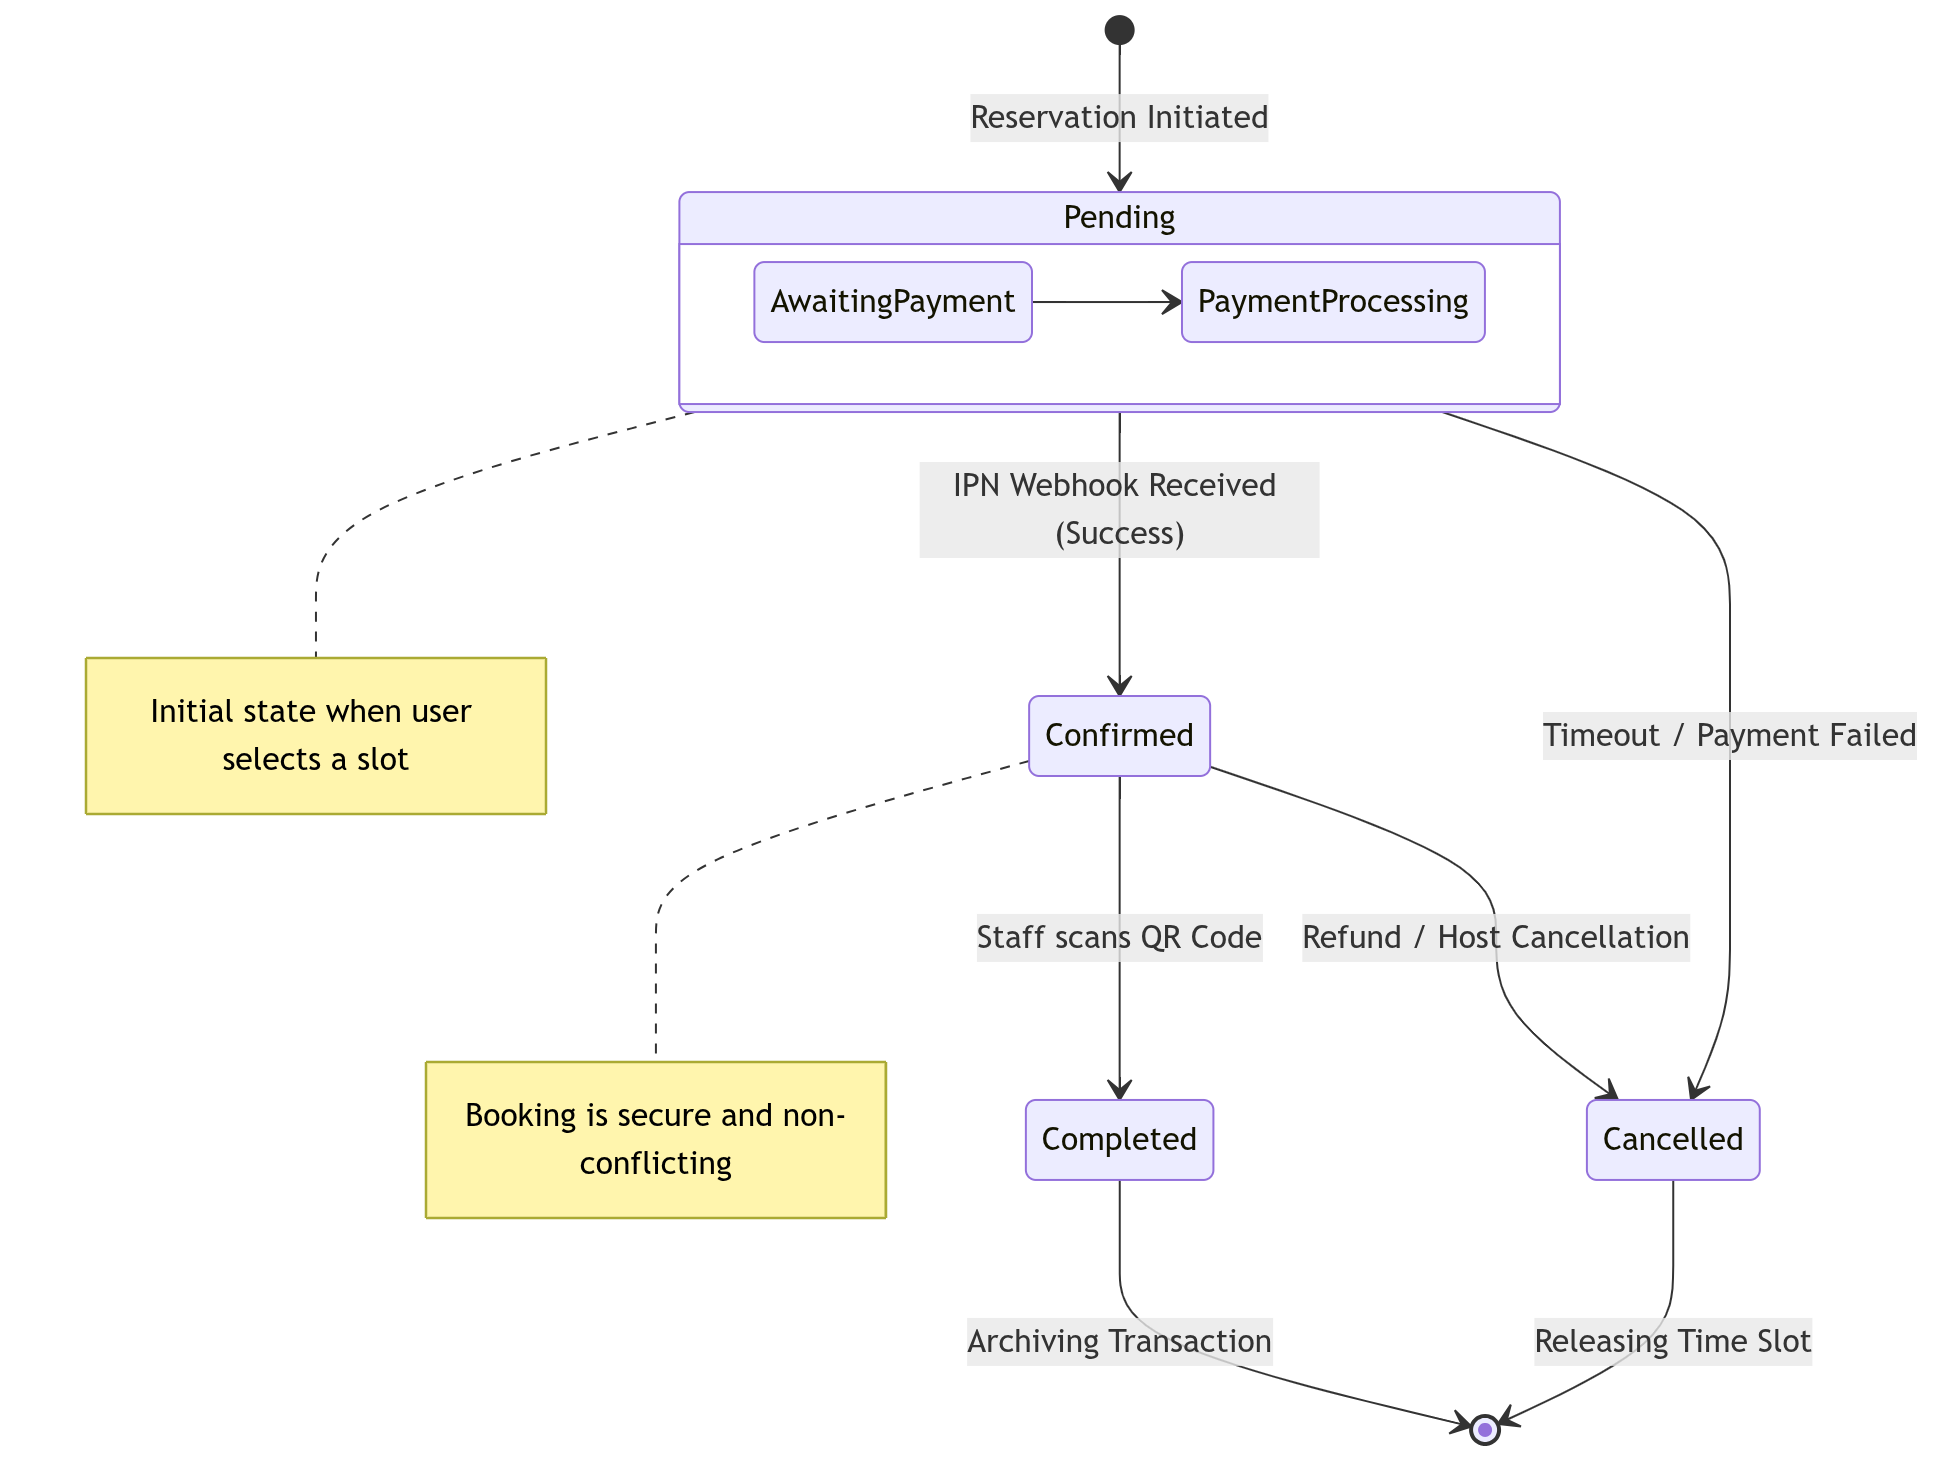
\includegraphics[width=0.7\textwidth]{Figures/booking_lifecycle.png}
    \caption{UML State Machine: The Booking Lifecycle and State Transitions}
    \label{fig:lifecycle}
\end{figure}

The \textbf{Booking Lifecycle} (Figure \ref{fig:lifecycle}) illustrates how the system manages transitions from the initial "Pending" state to the final "Completed" or "Cancelled" states, ensuring data consistency during concurrent booking attempts.

\subsection{AI Integration: Implementing Function Calling}
The integration of Google Gemini 2.5 Flash is implemented in the \texttt{aiService.js} module. Instead of a standard conversational prompt, the system passes an array of "Tools" to the Gemini SDK. 

One such tool is the \texttt{check\_availability} function. The JSON schema provided to the AI describes this function:
\begin{verbatim}
{
  "name": "check_availability",
  "description": "Checks if any fields are available 
                  at a given time.",
  "parameters": {
    "type": "object",
    "properties": {
      "time": { "type": "string", "description": "Time in HH:mm" },
      "date": { "type": "string", 
                "description": "Date in YYYY-MM-DD" }
    },
    "required": ["time", "date"]
  }
}
\end{verbatim}


When the user asks, "Is there a field available at 5 PM today?", the LLM outputs a "function call" request. The Node.js server intercepts this, parses the \texttt{time} ("17:00") and \texttt{date} parameters, queries the database to find unoccupied fields, and feeds the resulting array back to the LLM. The LLM then generates a human-readable response based on that array.

\subsection{Mobile App Implementation: Capacitor Hardware Bridge}
To bridge the web software with physical hardware, the \texttt{android-tenant} directory contains an Ionic Capacitor project. Capacitor wraps the standard HTML/JS web files into an Android APK.

To implement the rapid check-in feature, the native Camera plugin is invoked via JavaScript. Similarly, for wireless printing, the platform uses a unified interface:
\begin{verbatim}
// src/public/js/shared.js
function doRealPrint(htmlContent) {
  if (window.cordova && window.cordova.plugins 
      && window.cordova.plugins.printer) {
    window.cordova.plugins.printer.print(htmlContent, 
      { name: 'Invoice' });
  } else {
    window.print();
  }
}
\end{verbatim}
This approach ensures that the same code works on both web browsers and native mobile applications, providing a seamless user experience across all devices.

\subsection{Architectural Optimization and Modularization}
A significant milestone in the system's development was the transition from a monolithic frontend structure to a modular, asset-driven architecture. Originally, the CSS and JavaScript were embedded directly within the portal HTML files, leading to large file sizes and code duplication.

To optimize the platform, a shared design system was established:
\begin{itemize}
    \item \textbf{shared.css:} Centralizes all UI tokens, color palettes, and common components (e.g., glassmorphism utilities), ensuring visual consistency across all portals.
    \item \textbf{shared.js:} Provides a unified set of utility functions for API communication, currency formatting, and real-time state management.
\end{itemize}
By extracting these shared components, the size of the HTML files was reduced by over 80\%, resulting in significantly faster page load times and easier source code maintenance.

\subsection{Real-time Notification Pipeline}
The notification system is implemented as a dedicated utility in \texttt{src/utils/\allowbreak pushNotifier.js}. It utilizes the Firebase Admin SDK to send targeted messages to specific devices. The flow involves retrieving the target user's registered FCM token from the database and dispatching a JSON payload containing the notification content.

\subsection{User Interface Showcasing}
The platform features a modern, responsive user interface designed with a "Mobile-First" philosophy. The following sections describe the core interfaces developed for the platform.

\textbf{1. Provider Admin Dashboard:} 
This interface allows for the centralized management of all SaaS tenants. It provides tools for subscription tracking and system-wide analytics. (Refer to the live demo for detailed interface interactions).

\textbf{2. Tenant Admin Portal:} 
The primary operating environment for football field owners. It features an interactive time-grid schedule and a real-time dashboard for daily revenue tracking.

\textbf{3. Customer Storefront:} 
A mobile-optimized web interface that allows customers to search for fields and chat with the AI assistant. It integrates a seamless QR ticket display after successful payment.

% Note: Detailed UI screenshots are available in the accompanying digital documentation and live system demonstration.